\section{Finite bounds and proofs}\label{sec:finite}
Let $d\ge2$, $p\ge1$ and $\beta>0$ be fixed. The target is the normalized exponential-weighted mean on $\Sphere$ with values in $\Ball$. The budget $r_*$ counts persistent real coordinates of a deterministic encoder that is continuous on each fixed-length prefix. The budget $\rf$ supplies the key and rotation history for free. All accuracy statements below use the Euclidean norm, all finite histories and independently chosen queries. This section proves both continuous-state constants. It also gives an exact converse at zero error.

For $L\ge1$ let $D=D_{d,L}$ be the dimension of spherical polynomials of degree at most $L$. Define
\begin{align}
 c_{d,0}&=1, &
 c_{d,\ell}&=\frac{\beta^\ell}{d(d+2)\cdots(d+2\ell-2)}\quad(\ell\ge1),&
 \low&=\min\{1,c_{d,L}\}.\label{eq:spectralconst}
\end{align}
For $m\ge0$ put $\delta_m=\Pr\{\operatorname{Poisson}(2\beta)>m\}$.

\begin{theorem}[Finite inequalities]\label{thm:finite}
For every $m\ge0$ and $L\ge1$ the following implications hold.
\begin{align}
 2\delta_m/(1-\delta_m)\le\eps
 &\ \Longrightarrow\ r_*(\eps)\le(p+1)D_{d,m},\label{eq:upper}\\
 \eps<e^{-3\beta}\low/(8\sqrt D)
 &\ \Longrightarrow\ r_*(\eps)\ge(p+1)D-1,\label{eq:lower}\\
 \delta_m\le\eps
 &\ \Longrightarrow\ \rf(\eps)\le pD_{d,m},\label{eq:freeup}\\
 \eps<e^{-\beta}\low/(2\sqrt D)
 &\ \Longrightarrow\ \rf(\eps)\ge pD.\label{eq:freelow}
\end{align}
The lower bounds use identity rotations. The upper bounds allow any supplied rotations and any fixed continuous orthogonal representation on values.
\end{theorem}

\subsection{Positive polynomial moments}\label{sec:upper}
Set $P_m(t)=e^{-\beta}\sum_{a=0}^m [\beta(1+t)]^a/a!$. For $-1\le t\le1$, the ratio $P_m(t)/e^{\beta t}$ equals the probability that a Poisson variable of mean $\beta(1+t)$ is at most $m$. Hence $1-\delta_m\le P_m(t)/e^{\beta t}\le1$. If $\widetilde Z,\widetilde N$ are the two sums computed with $P_m$, then
\begin{equation}
 |Z-\widetilde Z|\le\delta_m Z,\qquad
 \norm{N-\widetilde N}_2\le\delta_m Z,\qquad
 \widetilde Z\ge(1-\delta_m)Z>0.\label{eq:uniform}
\end{equation}
Writing the difference of normalized outputs over $\widetilde Z$, and using $\norm{N/Z}_2\le1$, proves the error in \eqref{eq:upper}. Replacing $\widetilde Z$ by $Z$ proves the error in \eqref{eq:freeup}.

Use probability surface measure $\omega$. Choose real orthonormal spherical harmonics through degree $m$, concatenate them into a column $Y(k)$ and put $w(v)=(1,v^\top)^\top$. Harmonic decomposition of homogeneous polynomials gives
\[
 D_{d,m}=\binom{m+d-1}{d-1}+\binom{m+d-2}{d-1}.
\]
Indeed, the degree-$\ell$ harmonic dimension is the difference between the dimensions of homogeneous polynomials of degrees $\ell$ and $\ell-2$, with negative degrees empty. Summation telescopes \cite{atkinson}. For each $q$, the function $k\mapsto P_m(\ang qk)$ has expansion $a(q)^\top Y(k)$ in that basis. The moment matrix
$M=\sum_iY(k_i)w(v_i)^\top$ recovers both sums via $a(q)^\top M$. For a rotation $R$, write $Y(Rk)=U(R)Y(k)$ and $B(R)=\operatorname{diag}(1,\rho(R))$. The update is
\begin{equation}
 M_{t}=U(R_t) M_{t-1} B(R_t)^\top+Y(k_t)w(v_t)^\top,\qquad M_0=0.
 \label{eq:update}
\end{equation}
Each finite-prefix state map is continuous. The frame is already incorporated in $M_t$. There are $(p+1)D_{d,m}$ entries, or $pD_{d,m}$ if the mass is computed from free keys. For a nonnegative integer Poisson variable $X$ of mean $2\beta$,
$\mathbf1_{X\ge m+1}\le\binom{X}{m+1}$ and hence $\delta_m\le(2\beta)^{m+1}/(m+1)!$.

\subsection{A spectral estimate on a finite design}\label{sec:spectral}
Fix a spherical $2L$-design $x_1,\ldots,x_H$ with equal weights. Existence follows from \cite{design}. On the circle a regular polygon with more than $2L$ vertices suffices. Let $V_{ia}=Y_a(x_i)$ for the harmonics through degree $L$. Design exactness applied to products gives $V^\top V/H=I_D$. Rotation invariance makes $\sum_aY_a(x)^2$ constant, and its integral is $D$. Thus $\norm{Y(x)}_2=\sqrt D$. On grid vectors use $\ang fg_H=H^{-1}\sum_i f_i g_i$ and let $K_{ji}=H^{-1}\K(x_j,x_i)$.

\begin{lemma}[Visible low degrees]\label{lem:spectral}
If $g$ is in the column space of $V$, then $\norm{Kg}_H\ge\low\norm g_H$. The squared bounds add across vector components.
\end{lemma}
\begin{proof}
First truncate the exponential at degree $L$ in the unshifted variable. For each $a$, the kernel $(x^\top y)^a$ is positive semidefinite since it is the inner product of $x^{\otimes a}$ and $y^{\otimes a}$. The omitted exponential tail is therefore a positive semidefinite matrix on the grid, by convergence of finite sums.

For a harmonic homogeneous polynomial $h_\ell$ of degree $\ell\le L$, design integration of $(x^\top y)^a h_\ell(y)$ is exact for $a\le L$. Its sphere integral is a scalar multiple of $h_\ell(x)$ on $\Sphere$. To see both the sign and normalization, represent $h_\ell$ by a symmetric trace-free tensor. The degree-$2j$ moment of a uniform point $y$ is the sum of all Kronecker-delta pairings divided by $d(d+2)\cdots(d+2j-2)$. Odd moments vanish. This follows by writing a standard Gaussian as its independent radius and uniform direction, expanding its moment generating function, and using $\mathbb E\norm G^{2j}=d(d+2)\cdots(d+2j-2)$. A pairing of two tensor indices of $h_\ell$ vanishes by tracelessness. Each surviving term contracts all $\ell$ indices with copies of $x$ and pairs the remaining copies among themselves. Its value is $h_\ell(x)\norm x^{a-\ell}$, with a positive prefactor. At $a=\ell$ there are exactly $\ell!$ surviving pairings. The degree-zero calculation uses the empty product.

After multiplication by $\beta^a/a!$, the truncated kernel therefore has eigenvalue at least $c_{d,\ell}$ on the sampled degree-$\ell$ harmonics. These spaces are orthogonal in the grid norm. The ratio $c_{d,\ell+1}/c_{d,\ell}=\beta/(d+2\ell)$ decreases in $\ell$, so the minimum through degree $L$ is attained at an endpoint. Adding the positive semidefinite tail gives $\ang{g}{Kg}_H\ge\low\norm g_H^2$ on the sampled subspace. Cauchy--Schwarz gives the stated norm inequality even if $Kg$ leaves that subspace.
\end{proof}

\subsection{Independent mass and value perturbations}\label{sec:perturb}
Choose a scalar spherical polynomial $u$ with zero constant harmonic coefficient and $p$ spherical polynomials $f=(f_1,\ldots,f_p)$ allowing constants, all of degree at most $L$. The combined vector of coefficients $\theta$ ranges over the Euclidean unit sphere in $\R^M$, where $M=(p+1)D-1$. Write $u_i=u(x_i)$, $f_i=f(x_i)$ and $a=1/(2\sqrt D)$. Isometry on the design gives $\norm u_H^2+\sum_j\norm{f_j}_H^2=1$. Pointwise, $|u_i|\le\sqrt D$ and $\norm{f_i}_2\le\sqrt D$. Form a weighted prefix
\begin{equation}
 w_i=(1+a u_i)/H,\qquad v_i= a f_i/(1+a u_i).
 \label{eq:weights}
\end{equation}
The weights sum to one and are strictly positive. Values lie in the unit ball. At a grid query the antipodal prefixes have masses $d_0\pm z$ and numerators $\pm X$, where $d_0=(K\mathbf1)_j$, $z=a(Ku)_j$, and $X=a(Kf)_j$. By Lemma~\ref{lem:spectral} and averaging, some $j$ satisfies
\begin{equation}
 z^2+\norm X_2^2\ge a^2\low^2.\label{eq:signal}
\end{equation}

Fix a unit vector $e\in\R^p$ and a suffix key $k_*$ in advance. At the selected query let $b=\K(x_j,k_*)$ and $A=d_0+b$. Each choice of sign specifies a common suffix for the antipodal pair. For the resulting differences $\Delta_\sigma$ of the two outputs,
\begin{align}
 \Delta_\sigma&=\frac{X+\sigma be}{A+z}-\frac{-X+\sigma be}{A-z}
 =\frac{2(AX-\sigma bze)}{A^2-z^2},\nonumber\\
 \max_{\sigma=\pm1}\norm{\Delta_\sigma}_2
 &\ge \frac{2\sqrt{A^2\norm X_2^2+b^2z^2}}{A^2-z^2}
 \ge \frac{e^{-3\beta}}2\sqrt{\norm X_2^2+z^2}.
 \label{eq:twosigns}
\end{align}
The first inequality is the root-mean-square bound over the signs. The second uses $0<b\le A\le 2e^\beta$, $b\ge e^{-\beta}$ and $A>|z|$. Consequently the ideal separation for some query and sign is at least $g=e^{-3\beta}\low/(4\sqrt D)$.

\subsection{Fixed-length realization by ordinary tokens}\label{sec:realization}
\begin{lemma}[Uniform continuous realization]\label{lem:realize}
Let a compact parameter space index finitely many fixed keys on a path-connected sphere, strictly positive continuous weights summing to one and continuous values in $\Ball$. For every $\eta>0$ there is a single integer $n$ and a continuous map from the parameter space to $n$ ordinary key--value tokens, whose normalized mass and numerator sums approximate the weighted profiles within $\eta$ at every query.
\end{lemma}
\begin{proof}
Choose fixed continuous arcs joining consecutive keys in a cycle. Assign total time $1-\tau$ to plateaus and $\tau$ to the arcs, with plateau $i$ of duration $(1-\tau)w_i(\theta)$ and each arc of duration $\tau/H$. On a plateau keep the key and value fixed, and on an arc interpolate its endpoint values linearly. Compactness and positivity bound plateau durations away from zero. The pieces match at moving endpoints, giving a jointly continuous path $(k_\theta(s),v_\theta(s))$ on the compact product of parameters and $[0,1]$. For the scalar and vector integrands $\K(q,k_\theta(s))$ and $\K(q,k_\theta(s))v_\theta(s)$, the plateau contribution is exactly $1-\tau$ times the required weighted profile. The integral differs from the target by at most $2\tau e^\beta$ in either norm. Choose $\tau$ to make this less than $\eta/2$.

Uniform continuity jointly in $s,\theta,q$ then gives an equal-step midpoint Riemann sum of error less than $\eta/2$ for one $n$, simultaneously for all parameters and queries. The $n$ midpoint samples have unit token weight, normalized by $n$ in the comparison. Each sample depends continuously on $\theta$. Prefix queries and rotations may be fixed independently of the parameter.
\end{proof}

\paragraph{From a collision to a contradiction.}
Assume $2\eps<g$ and choose $\eta$ so that $g-2\eta e^\beta>2\eps$. Apply Lemma~\ref{lem:realize} to \eqref{eq:weights}. If $r<M$, the realized prefix state is a continuous map $S^{M-1}\to\R^r$. By Borsuk--Ulam \cite{borsuk}, padding the codomain with zeros if needed, some antipodal parameters have the same state. Choose their distinguishing design query and sign. Append $n$ copies of $k_*$ carrying the common value $\sigma e$, with identity rotations, fixed intermediate queries and the selected final query. Dividing the two prefix and suffix sums by $n$ makes the suffix mass exactly $b$. For each of the two prefixes the realized output differs from its ideal one by at most $\eta e^\beta$: the total denominator is at least $2e^{-\beta}$, the ideal output norm is at most one, and the two profile errors are each at most $\eta$. The realized outputs are thus separated by more than $2\eps$. The identical states and identical future force identical predictions, contradicting the triangle inequality. This proves \eqref{eq:lower}. The length is chosen before the collision. The query and sign are chosen afterward.

\paragraph{An explicit sufficient horizon.}
For the spherical construction, choose arcs of length at most $\pi$. The scalar integrand on each arc has total variation at most $\pi\beta e^\beta$, uniformly in $q$. The vector integrand has variation at most $e^\beta(\pi\beta+2)$ by the product rule for variation, since a straight segment between values has length at most two. Plateaus add zero variation. For any continuous vector-valued path of total variation $V$, the norm of the midpoint quadrature error is at most $V/n$: bound the error on each subinterval by its length times its variation and sum. Thus either profile error is at most
\[
 2\tau e^\beta+H e^\beta(\pi\beta+2)/n.
\]
With $\eta=(g-2\eps)e^{-\beta}/4$, any $0<\tau\le\min\{1/2,\eta/(4e^\beta)\}$ and $n\ge 2H e^\beta(\pi\beta+2)/\eta$ suffice. This gives a finite counterexample of at most $2n$ tokens for every encoder excluded by \eqref{eq:lower}, with $n$ chosen as the ceiling of the displayed threshold. The design, arc paths and length can all be fixed before examining the encoder.

\paragraph{The free-key converse.}
Use the same design, with its $H$ ordinary keys in a fixed order, each once, and set $v_i=f(x_i)/\sqrt D$. Here all $pD$ coefficients of the vector polynomial $f$ lie on their unit sphere, and $\norm{v_i}_2\le1$. For $r<pD$ some antipodal pair has identical paid state. The key-only history is identical as well. Lemma~\ref{lem:spectral} gives a grid query with $\norm{(Kf)_j}_2\ge\low$. Append $H$ copies of the same key with zero value and read that query. The two exact outputs differ by
$2\norm{(Kf)_j}_2/(\sqrt D\,(d_0+b))\ge e^{-\beta}\low/\sqrt D$.
This contradicts accuracy when the strict inequality in \eqref{eq:freelow} holds. The suffix permits the final query to be selected after the prefix collision even in an update-then-read implementation.

\subsection{Asymptotic inversion}\label{sec:limit}
The product in \eqref{eq:spectralconst} is $2^L\Gamma(L+d/2)/\Gamma(d/2)$. Stirling's formula gives
\[
 \log\!\left(\frac{8e^{3\beta}\sqrt{D_{d,L}}}{\lambda_{d,L}}\right)
 =L\log L+O_{d,\beta}(L).
\]
The free-key threshold has the same leading logarithm. For fixed $0<u<1$ and $T=\log(1/\eps)$ take $L=\lfloor(1-u)T/\log T\rfloor$. Then $L\log L=(1-u+o(1))T$, activating both lower bounds for small $\eps$. For $m=\lceil(1+u)T/\log T\rceil$ the factorial upper bound on $\delta_m$ gives $\log\delta_m\le-(1+u+o(1))T$. Both upper bounds apply. Dividing by $(T/\log T)^{d-1}$ and using $D_{d,L}\sim2L^{d-1}/(d-1)!$ puts the liminf and limsup between the corresponding multiples of $(1-u)^{d-1}$ and $(1+u)^{d-1}$. Sending $u$ to zero proves both limits.

\section{Exact future equivalence}\label{sec:exact}
For a finite prefix in its current frame let $\mu=\sum_i\delta_{k_i}$ and $\nu=\sum_i v_i\delta_{k_i}$, the latter a vector measure. For each $q$, append the same key of known weight $b>0$ and use values $0$ and $e$ in two separate tests. If outputs agree between prefixes on both tests, the difference $be/(Z+b)$ agrees between them. It determines $Z$ and then $N$ at that query. Equality of future readouts therefore implies equality of all exponential transforms of $\mu$ and each coordinate of $\nu$.

Here is a finite-support injectivity proof. If a signed difference $\xi=\sum_{i=1}^J c_i\delta_{x_i}$ at distinct $x_i$ has identically zero transform, integrate its transform against $\xi$. Absolute convergence permits the expansion
\begin{equation}
 0=\sum_{i,j}c_i c_j e^{\beta\ang{x_i}{x_j}}
 =\sum_{a=0}^{\infty}\frac{\beta^a}{a!}
 \left\|\sum_i c_i x_i^{\otimes a}\right\|_2^2.\label{eq:ident}
\end{equation}
All tensor moments vanish, hence $\xi$ annihilates every polynomial. The polynomial
$\prod_{j\ne i}(1-x^\top x_j)/(1-x_i^\top x_j)$ is one at $x_i$ and zero at the other support points. Thus every $c_i=0$. This argument is also consistent with the general theory of universal dot-product kernels \cite{universal}. Conversely, common updates push equal measures forward by the same rotation, rotate the vector masses by $\rho$, and add the same atom. Equal measures remain equal and give identical future readouts.

\begin{corollary}[Exact prefixes of length $n$]\label{cor:exact}
For $n\ge1$, a continuous encoder whose state after $n$ tokens supports exact answers on every common one-token continuation needs at least $n(d-1+p)$ real coordinates.
\end{corollary}
\begin{proof}
Choose $n$ disjoint open key patches, each admitting a Euclidean chart, and allow each value to range over the open unit ball. Distinct inputs in this family give different pairs of measures, since the patches label the keys. The two-probe argument forces the state map to be injective on an open set of dimension $m=n(d-1+p)$. A small sphere inside the open set has dimension $m-1$. For an output dimension below $m$, Borsuk--Ulam forces an antipodal collision on this sphere. This proves the lower bound.
\end{proof}

\section{Reproducible calculations and verification scope}\label{sec:checks}
For the five-token example, at $q=x$ the prefix masses are $13/2$ and $7/2$. After $j$ perpendicular keys of value one the corresponding outputs are $j/(13/2+j)$ and $j/(7/2+j)$. At $j=1$ their gap is $4/45$. The plotted inputs use exact rational values. For the finite-dimension plot we set $\eps=10^{-k}$ and enumerate integer degrees. A lower degree is admissible under the strict inequality in \eqref{eq:lower}. For the upper curve we use the sufficient bound $(2\beta)^{m+1}/(m+1)!\le\eps/(2+\eps)$ rather than an estimate of a tiny tail probability. Logarithms keep the comparisons numerically stable. The zero lower bound is always available. The notebook includes a rational-arithmetic cross-check of selected degrees.

The numerical checks use a regular polygon on the circle, the six vertices of an octahedron on $\mathbb S^2$ ($L=1$), and the 24-cell on $\mathbb S^3$ ($L=2$). They compare the sampled quadratic form to the proved lower bound. On the circle a separate finite Fourier recurrence is compared to dense polynomial attention with rotating keys and values. All inputs and tests are deterministic. They verify implementations in these examples.

The ancillary Lean 4.19.0 sources and their archived checker transcript cover the additive two-probe identity, the vector two-sign calculation, the collision implication and the exact five-token example. The spherical spectral estimate, realization by unit tokens, Borsuk--Ulam lower bound and dimension limits are proved in the text. The notebook verifies the archived source hashes and runs the numerical checks independently.

\begin{figure}[ht]\centering
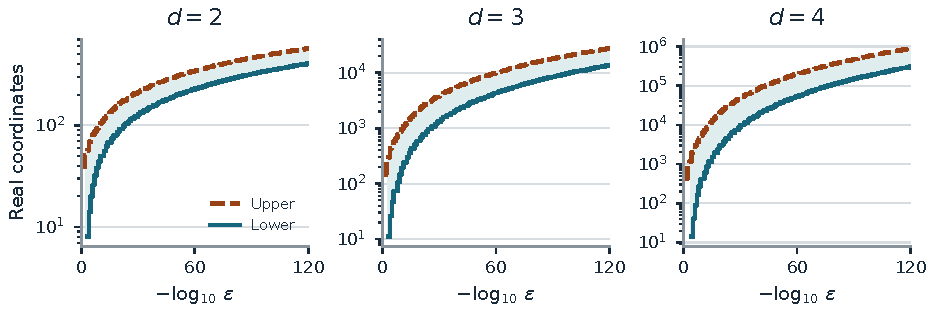
\includegraphics[width=.92\linewidth]{figures/dimension.pdf}
\caption{Finite, certified intervals for continuous state dimension at $p=2$ and $\beta=1$. The constructive and obstruction degrees are computed independently. Horizontal coordinates give the requested number of decimal digits of accuracy.}\label{fig:bounds}
\end{figure}
